% SOURCE: ../../edit-harness/results/merging/RG_gain_law_20260715.json + ../../edit-harness/results/merging/RG_crossterm_alignment_ALL_REFIX20260801.json
% !TEX encoding = UTF-8 Unicode
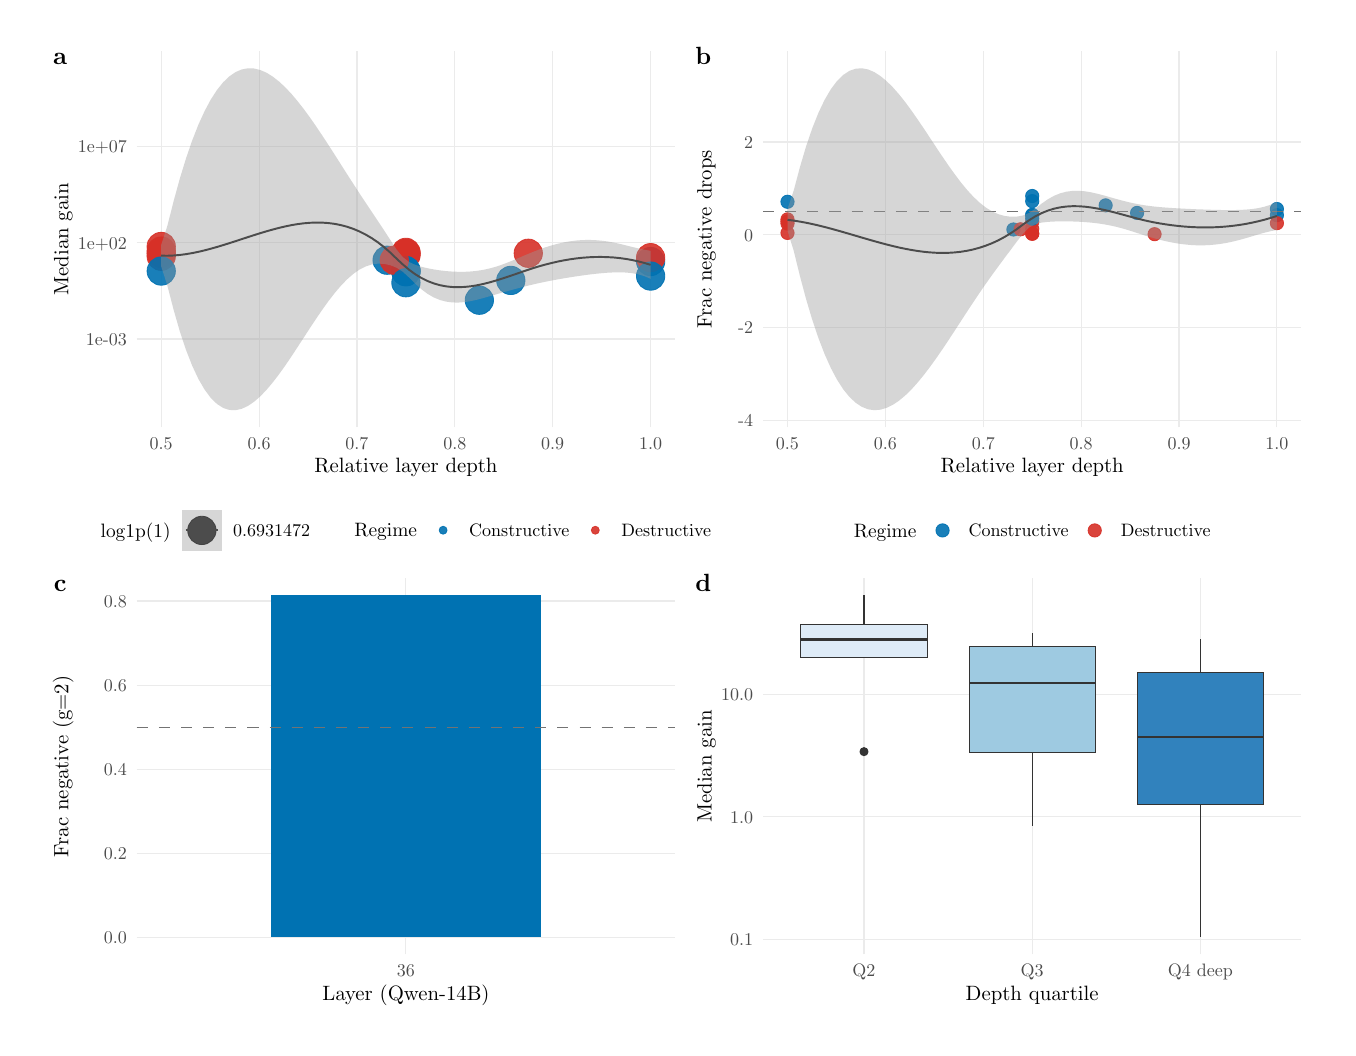
\begin{tikzpicture}[x=1pt,y=1pt]
\definecolor{fillColor}{RGB}{255,255,255}
\path[use as bounding box,fill=fillColor,fill opacity=0.00] (0,0) rectangle (469.75,361.35);
\begin{scope}
\path[clip] (  0.00,  0.00) rectangle (469.75,361.35);
\definecolor{drawColor}{RGB}{255,255,255}
\definecolor{fillColor}{RGB}{255,255,255}

\path[draw=drawColor,line width= 0.6pt,line join=round,line cap=round,fill=fillColor] (  0.00,  0.00) rectangle (469.76,361.35);
\end{scope}
\begin{scope}
\path[clip] (  5.50,165.37) rectangle (237.95,355.85);
\definecolor{fillColor}{RGB}{255,255,255}

\path[fill=fillColor] (  5.50,165.37) rectangle (237.95,355.85);
\end{scope}
\begin{scope}
\path[clip] (237.95,165.37) rectangle (464.25,355.85);
\definecolor{fillColor}{RGB}{255,255,255}

\path[fill=fillColor] (237.95,165.37) rectangle (464.25,355.85);
\end{scope}
\begin{scope}
\path[clip] (  5.50,  5.50) rectangle (237.95,165.37);
\definecolor{fillColor}{RGB}{255,255,255}

\path[fill=fillColor] (  5.50,  5.50) rectangle (237.95,165.37);
\end{scope}
\begin{scope}
\path[clip] (237.95,  5.50) rectangle (464.25,165.37);
\definecolor{fillColor}{RGB}{255,255,255}

\path[fill=fillColor] (237.95,  5.50) rectangle (464.25,165.37);
\end{scope}
\begin{scope}
\path[clip] ( 39.41,216.94) rectangle (233.95,352.85);
\definecolor{drawColor}{gray}{0.92}

\path[draw=drawColor,line width= 0.4pt,line join=round] ( 39.41,248.86) --
	(233.95,248.86);

\path[draw=drawColor,line width= 0.4pt,line join=round] ( 39.41,283.60) --
	(233.95,283.60);

\path[draw=drawColor,line width= 0.4pt,line join=round] ( 39.41,318.34) --
	(233.95,318.34);

\path[draw=drawColor,line width= 0.4pt,line join=round] ( 48.26,216.94) --
	( 48.26,352.85);

\path[draw=drawColor,line width= 0.4pt,line join=round] ( 83.63,216.94) --
	( 83.63,352.85);

\path[draw=drawColor,line width= 0.4pt,line join=round] (118.99,216.94) --
	(118.99,352.85);

\path[draw=drawColor,line width= 0.4pt,line join=round] (154.36,216.94) --
	(154.36,352.85);

\path[draw=drawColor,line width= 0.4pt,line join=round] (189.73,216.94) --
	(189.73,352.85);

\path[draw=drawColor,line width= 0.4pt,line join=round] (225.10,216.94) --
	(225.10,352.85);
\definecolor{drawColor}{RGB}{215,48,39}
\definecolor{fillColor}{RGB}{215,48,39}

\path[draw=drawColor,draw opacity=0.90,line width= 0.3pt,line join=round,line cap=round,fill=fillColor,fill opacity=0.90] (136.68,279.06) circle (  5.12);

\path[draw=drawColor,draw opacity=0.90,line width= 0.3pt,line join=round,line cap=round,fill=fillColor,fill opacity=0.90] (136.68,279.67) circle (  5.12);

\path[draw=drawColor,draw opacity=0.90,line width= 0.3pt,line join=round,line cap=round,fill=fillColor,fill opacity=0.90] (180.89,279.83) circle (  5.12);

\path[draw=drawColor,draw opacity=0.90,line width= 0.3pt,line join=round,line cap=round,fill=fillColor,fill opacity=0.90] ( 48.26,282.28) circle (  5.12);

\path[draw=drawColor,draw opacity=0.90,line width= 0.3pt,line join=round,line cap=round,fill=fillColor,fill opacity=0.90] (136.68,280.16) circle (  5.12);

\path[draw=drawColor,draw opacity=0.90,line width= 0.3pt,line join=round,line cap=round,fill=fillColor,fill opacity=0.90] (136.68,279.79) circle (  5.12);
\definecolor{drawColor}{RGB}{0,114,178}
\definecolor{fillColor}{RGB}{0,114,178}

\path[draw=drawColor,draw opacity=0.90,line width= 0.3pt,line join=round,line cap=round,fill=fillColor,fill opacity=0.90] (225.10,276.85) circle (  5.12);
\definecolor{drawColor}{RGB}{215,48,39}
\definecolor{fillColor}{RGB}{215,48,39}

\path[draw=drawColor,draw opacity=0.90,line width= 0.3pt,line join=round,line cap=round,fill=fillColor,fill opacity=0.90] (225.10,278.24) circle (  5.12);
\definecolor{drawColor}{RGB}{0,114,178}
\definecolor{fillColor}{RGB}{0,114,178}

\path[draw=drawColor,draw opacity=0.90,line width= 0.3pt,line join=round,line cap=round,fill=fillColor,fill opacity=0.90] (225.10,271.59) circle (  5.12);
\definecolor{drawColor}{RGB}{215,48,39}
\definecolor{fillColor}{RGB}{215,48,39}

\path[draw=drawColor,draw opacity=0.90,line width= 0.3pt,line join=round,line cap=round,fill=fillColor,fill opacity=0.90] ( 48.26,279.77) circle (  5.12);
\definecolor{drawColor}{RGB}{0,114,178}
\definecolor{fillColor}{RGB}{0,114,178}

\path[draw=drawColor,draw opacity=0.90,line width= 0.3pt,line join=round,line cap=round,fill=fillColor,fill opacity=0.90] (136.68,273.30) circle (  5.12);

\path[draw=drawColor,draw opacity=0.90,line width= 0.3pt,line join=round,line cap=round,fill=fillColor,fill opacity=0.90] (174.58,270.02) circle (  5.12);

\path[draw=drawColor,draw opacity=0.90,line width= 0.3pt,line join=round,line cap=round,fill=fillColor,fill opacity=0.90] (136.68,273.12) circle (  5.12);
\definecolor{drawColor}{RGB}{215,48,39}
\definecolor{fillColor}{RGB}{215,48,39}

\path[draw=drawColor,draw opacity=0.90,line width= 0.3pt,line join=round,line cap=round,fill=fillColor,fill opacity=0.90] ( 48.26,280.62) circle (  5.12);
\definecolor{drawColor}{RGB}{0,114,178}
\definecolor{fillColor}{RGB}{0,114,178}

\path[draw=drawColor,draw opacity=0.90,line width= 0.3pt,line join=round,line cap=round,fill=fillColor,fill opacity=0.90] (136.68,273.59) circle (  5.12);

\path[draw=drawColor,draw opacity=0.90,line width= 0.3pt,line join=round,line cap=round,fill=fillColor,fill opacity=0.90] (136.68,273.44) circle (  5.12);
\definecolor{drawColor}{RGB}{215,48,39}
\definecolor{fillColor}{RGB}{215,48,39}

\path[draw=drawColor,draw opacity=0.90,line width= 0.3pt,line join=round,line cap=round,fill=fillColor,fill opacity=0.90] ( 48.26,278.74) circle (  5.12);
\definecolor{drawColor}{RGB}{0,114,178}
\definecolor{fillColor}{RGB}{0,114,178}

\path[draw=drawColor,draw opacity=0.90,line width= 0.3pt,line join=round,line cap=round,fill=fillColor,fill opacity=0.90] (129.88,277.32) circle (  5.12);
\definecolor{drawColor}{RGB}{215,48,39}
\definecolor{fillColor}{RGB}{215,48,39}

\path[draw=drawColor,draw opacity=0.90,line width= 0.3pt,line join=round,line cap=round,fill=fillColor,fill opacity=0.90] (132.47,277.32) circle (  5.12);
\definecolor{drawColor}{RGB}{0,114,178}
\definecolor{fillColor}{RGB}{0,114,178}

\path[draw=drawColor,draw opacity=0.90,line width= 0.3pt,line join=round,line cap=round,fill=fillColor,fill opacity=0.90] (163.21,262.86) circle (  5.12);

\path[draw=drawColor,draw opacity=0.90,line width= 0.3pt,line join=round,line cap=round,fill=fillColor,fill opacity=0.90] ( 48.26,273.40) circle (  5.12);

\path[draw=drawColor,draw opacity=0.90,line width= 0.3pt,line join=round,line cap=round,fill=fillColor,fill opacity=0.90] (136.68,269.18) circle (  5.12);
\definecolor{fillColor}{RGB}{153,153,153}

\path[fill=fillColor,fill opacity=0.40] ( 48.26,282.89) --
	( 50.49,289.77) --
	( 52.73,298.62) --
	( 54.97,306.77) --
	( 57.21,314.09) --
	( 59.45,320.59) --
	( 61.69,326.28) --
	( 63.93,331.19) --
	( 66.16,335.36) --
	( 68.40,338.82) --
	( 70.64,341.61) --
	( 72.88,343.75) --
	( 75.12,345.29) --
	( 77.36,346.25) --
	( 79.60,346.67) --
	( 81.83,346.59) --
	( 84.07,346.04) --
	( 86.31,345.06) --
	( 88.55,343.67) --
	( 90.79,341.92) --
	( 93.03,339.84) --
	( 95.27,337.47) --
	( 97.50,334.83) --
	( 99.74,331.96) --
	(101.98,328.91) --
	(104.22,325.70) --
	(106.46,322.36) --
	(108.70,318.93) --
	(110.94,315.45) --
	(113.17,311.94) --
	(115.41,308.42) --
	(117.65,304.94) --
	(119.89,301.49) --
	(122.13,298.10) --
	(124.37,294.74) --
	(126.61,291.39) --
	(128.84,288.02) --
	(131.08,284.57) --
	(133.32,281.14) --
	(135.56,278.43) --
	(137.80,276.69) --
	(140.04,275.66) --
	(142.28,274.95) --
	(144.51,274.41) --
	(146.75,273.98) --
	(148.99,273.64) --
	(151.23,273.38) --
	(153.47,273.21) --
	(155.71,273.12) --
	(157.95,273.13) --
	(160.18,273.25) --
	(162.42,273.48) --
	(164.66,273.84) --
	(166.90,274.33) --
	(169.14,274.95) --
	(171.38,275.70) --
	(173.62,276.55) --
	(175.85,277.47) --
	(178.09,278.43) --
	(180.33,279.38) --
	(182.57,280.31) --
	(184.81,281.17) --
	(187.05,281.96) --
	(189.29,282.65) --
	(191.53,283.26) --
	(193.76,283.76) --
	(196.00,284.15) --
	(198.24,284.43) --
	(200.48,284.60) --
	(202.72,284.65) --
	(204.96,284.58) --
	(207.20,284.39) --
	(209.43,284.10) --
	(211.67,283.71) --
	(213.91,283.23) --
	(216.15,282.69) --
	(218.39,282.13) --
	(220.63,281.58) --
	(222.87,281.10) --
	(225.10,280.71) --
	(225.10,270.59) --
	(222.87,271.55) --
	(220.63,272.22) --
	(218.39,272.64) --
	(216.15,272.87) --
	(213.91,272.94) --
	(211.67,272.91) --
	(209.43,272.79) --
	(207.20,272.61) --
	(204.96,272.38) --
	(202.72,272.12) --
	(200.48,271.82) --
	(198.24,271.49) --
	(196.00,271.15) --
	(193.76,270.78) --
	(191.53,270.39) --
	(189.29,269.97) --
	(187.05,269.53) --
	(184.81,269.06) --
	(182.57,268.55) --
	(180.33,268.01) --
	(178.09,267.43) --
	(175.85,266.84) --
	(173.62,266.23) --
	(171.38,265.59) --
	(169.14,264.94) --
	(166.90,264.29) --
	(164.66,263.65) --
	(162.42,263.06) --
	(160.18,262.56) --
	(157.95,262.20) --
	(155.71,262.02) --
	(153.47,262.05) --
	(151.23,262.35) --
	(148.99,262.94) --
	(146.75,263.87) --
	(144.51,265.16) --
	(142.28,266.83) --
	(140.04,268.84) --
	(137.80,271.08) --
	(135.56,273.15) --
	(133.32,274.59) --
	(131.08,275.50) --
	(128.84,275.98) --
	(126.61,276.08) --
	(124.37,275.79) --
	(122.13,275.07) --
	(119.89,273.93) --
	(117.65,272.36) --
	(115.41,270.40) --
	(113.17,268.08) --
	(110.94,265.45) --
	(108.70,262.56) --
	(106.46,259.44) --
	(104.22,256.17) --
	(101.98,252.78) --
	( 99.74,249.33) --
	( 97.50,245.89) --
	( 95.27,242.49) --
	( 93.03,239.19) --
	( 90.79,236.06) --
	( 88.55,233.14) --
	( 86.31,230.48) --
	( 84.07,228.15) --
	( 81.83,226.19) --
	( 79.60,224.67) --
	( 77.36,223.63) --
	( 75.12,223.12) --
	( 72.88,223.21) --
	( 70.64,223.95) --
	( 68.40,225.38) --
	( 66.16,227.57) --
	( 63.93,230.57) --
	( 61.69,234.43) --
	( 59.45,239.20) --
	( 57.21,244.93) --
	( 54.97,251.67) --
	( 52.73,259.43) --
	( 50.49,268.10) --
	( 48.26,275.04) --
	cycle;

\path[] ( 48.26,282.89) --
	( 50.49,289.77) --
	( 52.73,298.62) --
	( 54.97,306.77) --
	( 57.21,314.09) --
	( 59.45,320.59) --
	( 61.69,326.28) --
	( 63.93,331.19) --
	( 66.16,335.36) --
	( 68.40,338.82) --
	( 70.64,341.61) --
	( 72.88,343.75) --
	( 75.12,345.29) --
	( 77.36,346.25) --
	( 79.60,346.67) --
	( 81.83,346.59) --
	( 84.07,346.04) --
	( 86.31,345.06) --
	( 88.55,343.67) --
	( 90.79,341.92) --
	( 93.03,339.84) --
	( 95.27,337.47) --
	( 97.50,334.83) --
	( 99.74,331.96) --
	(101.98,328.91) --
	(104.22,325.70) --
	(106.46,322.36) --
	(108.70,318.93) --
	(110.94,315.45) --
	(113.17,311.94) --
	(115.41,308.42) --
	(117.65,304.94) --
	(119.89,301.49) --
	(122.13,298.10) --
	(124.37,294.74) --
	(126.61,291.39) --
	(128.84,288.02) --
	(131.08,284.57) --
	(133.32,281.14) --
	(135.56,278.43) --
	(137.80,276.69) --
	(140.04,275.66) --
	(142.28,274.95) --
	(144.51,274.41) --
	(146.75,273.98) --
	(148.99,273.64) --
	(151.23,273.38) --
	(153.47,273.21) --
	(155.71,273.12) --
	(157.95,273.13) --
	(160.18,273.25) --
	(162.42,273.48) --
	(164.66,273.84) --
	(166.90,274.33) --
	(169.14,274.95) --
	(171.38,275.70) --
	(173.62,276.55) --
	(175.85,277.47) --
	(178.09,278.43) --
	(180.33,279.38) --
	(182.57,280.31) --
	(184.81,281.17) --
	(187.05,281.96) --
	(189.29,282.65) --
	(191.53,283.26) --
	(193.76,283.76) --
	(196.00,284.15) --
	(198.24,284.43) --
	(200.48,284.60) --
	(202.72,284.65) --
	(204.96,284.58) --
	(207.20,284.39) --
	(209.43,284.10) --
	(211.67,283.71) --
	(213.91,283.23) --
	(216.15,282.69) --
	(218.39,282.13) --
	(220.63,281.58) --
	(222.87,281.10) --
	(225.10,280.71);

\path[] (225.10,270.59) --
	(222.87,271.55) --
	(220.63,272.22) --
	(218.39,272.64) --
	(216.15,272.87) --
	(213.91,272.94) --
	(211.67,272.91) --
	(209.43,272.79) --
	(207.20,272.61) --
	(204.96,272.38) --
	(202.72,272.12) --
	(200.48,271.82) --
	(198.24,271.49) --
	(196.00,271.15) --
	(193.76,270.78) --
	(191.53,270.39) --
	(189.29,269.97) --
	(187.05,269.53) --
	(184.81,269.06) --
	(182.57,268.55) --
	(180.33,268.01) --
	(178.09,267.43) --
	(175.85,266.84) --
	(173.62,266.23) --
	(171.38,265.59) --
	(169.14,264.94) --
	(166.90,264.29) --
	(164.66,263.65) --
	(162.42,263.06) --
	(160.18,262.56) --
	(157.95,262.20) --
	(155.71,262.02) --
	(153.47,262.05) --
	(151.23,262.35) --
	(148.99,262.94) --
	(146.75,263.87) --
	(144.51,265.16) --
	(142.28,266.83) --
	(140.04,268.84) --
	(137.80,271.08) --
	(135.56,273.15) --
	(133.32,274.59) --
	(131.08,275.50) --
	(128.84,275.98) --
	(126.61,276.08) --
	(124.37,275.79) --
	(122.13,275.07) --
	(119.89,273.93) --
	(117.65,272.36) --
	(115.41,270.40) --
	(113.17,268.08) --
	(110.94,265.45) --
	(108.70,262.56) --
	(106.46,259.44) --
	(104.22,256.17) --
	(101.98,252.78) --
	( 99.74,249.33) --
	( 97.50,245.89) --
	( 95.27,242.49) --
	( 93.03,239.19) --
	( 90.79,236.06) --
	( 88.55,233.14) --
	( 86.31,230.48) --
	( 84.07,228.15) --
	( 81.83,226.19) --
	( 79.60,224.67) --
	( 77.36,223.63) --
	( 75.12,223.12) --
	( 72.88,223.21) --
	( 70.64,223.95) --
	( 68.40,225.38) --
	( 66.16,227.57) --
	( 63.93,230.57) --
	( 61.69,234.43) --
	( 59.45,239.20) --
	( 57.21,244.93) --
	( 54.97,251.67) --
	( 52.73,259.43) --
	( 50.49,268.10) --
	( 48.26,275.04);
\definecolor{drawColor}{gray}{0.30}

\path[draw=drawColor,line width= 0.7pt,line join=round] ( 48.26,278.96) --
	( 50.49,278.93) --
	( 52.73,279.02) --
	( 54.97,279.22) --
	( 57.21,279.51) --
	( 59.45,279.89) --
	( 61.69,280.35) --
	( 63.93,280.88) --
	( 66.16,281.47) --
	( 68.40,282.10) --
	( 70.64,282.78) --
	( 72.88,283.48) --
	( 75.12,284.20) --
	( 77.36,284.94) --
	( 79.60,285.67) --
	( 81.83,286.39) --
	( 84.07,287.10) --
	( 86.31,287.77) --
	( 88.55,288.40) --
	( 90.79,288.99) --
	( 93.03,289.52) --
	( 95.27,289.98) --
	( 97.50,290.36) --
	( 99.74,290.65) --
	(101.98,290.84) --
	(104.22,290.93) --
	(106.46,290.90) --
	(108.70,290.74) --
	(110.94,290.45) --
	(113.17,290.01) --
	(115.41,289.41) --
	(117.65,288.65) --
	(119.89,287.71) --
	(122.13,286.58) --
	(124.37,285.26) --
	(126.61,283.74) --
	(128.84,282.00) --
	(131.08,280.03) --
	(133.32,277.86) --
	(135.56,275.79) --
	(137.80,273.89) --
	(140.04,272.25) --
	(142.28,270.89) --
	(144.51,269.79) --
	(146.75,268.93) --
	(148.99,268.29) --
	(151.23,267.86) --
	(153.47,267.63) --
	(155.71,267.57) --
	(157.95,267.67) --
	(160.18,267.90) --
	(162.42,268.27) --
	(164.66,268.74) --
	(166.90,269.31) --
	(169.14,269.95) --
	(171.38,270.65) --
	(173.62,271.39) --
	(175.85,272.15) --
	(178.09,272.93) --
	(180.33,273.69) --
	(182.57,274.43) --
	(184.81,275.12) --
	(187.05,275.74) --
	(189.29,276.31) --
	(191.53,276.82) --
	(193.76,277.27) --
	(196.00,277.65) --
	(198.24,277.96) --
	(200.48,278.21) --
	(202.72,278.38) --
	(204.96,278.48) --
	(207.20,278.50) --
	(209.43,278.44) --
	(211.67,278.31) --
	(213.91,278.09) --
	(216.15,277.78) --
	(218.39,277.39) --
	(220.63,276.90) --
	(222.87,276.32) --
	(225.10,275.65);
\end{scope}
\begin{scope}
\path[clip] (  0.00,  0.00) rectangle (469.75,361.35);
\definecolor{drawColor}{gray}{0.30}

\node[text=drawColor,anchor=base east,inner sep=0pt, outer sep=0pt, scale=  0.65] at ( 35.81,246.62) {1e-03};

\node[text=drawColor,anchor=base east,inner sep=0pt, outer sep=0pt, scale=  0.65] at ( 35.81,281.36) {1e+02};

\node[text=drawColor,anchor=base east,inner sep=0pt, outer sep=0pt, scale=  0.65] at ( 35.81,316.10) {1e+07};
\end{scope}
\begin{scope}
\path[clip] (  0.00,  0.00) rectangle (469.75,361.35);
\definecolor{drawColor}{gray}{0.30}

\node[text=drawColor,anchor=base,inner sep=0pt, outer sep=0pt, scale=  0.65] at ( 48.26,208.87) {0.5};

\node[text=drawColor,anchor=base,inner sep=0pt, outer sep=0pt, scale=  0.65] at ( 83.63,208.87) {0.6};

\node[text=drawColor,anchor=base,inner sep=0pt, outer sep=0pt, scale=  0.65] at (118.99,208.87) {0.7};

\node[text=drawColor,anchor=base,inner sep=0pt, outer sep=0pt, scale=  0.65] at (154.36,208.87) {0.8};

\node[text=drawColor,anchor=base,inner sep=0pt, outer sep=0pt, scale=  0.65] at (189.73,208.87) {0.9};

\node[text=drawColor,anchor=base,inner sep=0pt, outer sep=0pt, scale=  0.65] at (225.10,208.87) {1.0};
\end{scope}
\begin{scope}
\path[clip] (  0.00,  0.00) rectangle (469.75,361.35);
\definecolor{drawColor}{RGB}{0,0,0}

\node[text=drawColor,anchor=base,inner sep=0pt, outer sep=0pt, scale=  0.75] at (136.68,200.44) {Relative layer depth};
\end{scope}
\begin{scope}
\path[clip] (  0.00,  0.00) rectangle (469.75,361.35);
\definecolor{drawColor}{RGB}{0,0,0}

\node[text=drawColor,rotate= 90.00,anchor=base,inner sep=0pt, outer sep=0pt, scale=  0.75] at ( 14.67,284.90) {Median gain};
\end{scope}
\begin{scope}
\path[clip] (  0.00,  0.00) rectangle (469.75,361.35);
\definecolor{drawColor}{RGB}{0,0,0}

\node[text=drawColor,anchor=base west,inner sep=0pt, outer sep=0pt, scale=  0.70] at ( 26.37,177.26) {log1p(1)};
\end{scope}
\begin{scope}
\path[clip] (  0.00,  0.00) rectangle (469.75,361.35);
\definecolor{drawColor}{RGB}{0,0,0}
\definecolor{fillColor}{RGB}{0,0,0}

\path[draw=drawColor,draw opacity=0.90,line width= 0.3pt,line join=round,line cap=round,fill=fillColor,fill opacity=0.90] ( 62.95,179.68) circle (  5.12);
\definecolor{fillColor}{RGB}{153,153,153}

\path[fill=fillColor,fill opacity=0.40] ( 55.64,172.37) rectangle ( 70.25,186.98);
\definecolor{drawColor}{gray}{0.30}

\path[draw=drawColor,line width= 0.7pt,line join=round] ( 57.10,179.68) -- ( 68.79,179.68);
\end{scope}
\begin{scope}
\path[clip] (  0.00,  0.00) rectangle (469.75,361.35);
\definecolor{drawColor}{RGB}{0,0,0}

\node[text=drawColor,anchor=base west,inner sep=0pt, outer sep=0pt, scale=  0.65] at ( 74.25,177.44) {0.6931472};
\end{scope}
\begin{scope}
\path[clip] (  0.00,  0.00) rectangle (469.75,361.35);
\definecolor{drawColor}{RGB}{0,0,0}

\node[text=drawColor,anchor=base west,inner sep=0pt, outer sep=0pt, scale=  0.70] at (118.05,177.34) {Regime};
\end{scope}
\begin{scope}
\path[clip] (  0.00,  0.00) rectangle (469.75,361.35);
\definecolor{drawColor}{RGB}{0,114,178}
\definecolor{fillColor}{RGB}{0,114,178}

\path[draw=drawColor,draw opacity=0.90,line width= 0.3pt,line join=round,line cap=round,fill=fillColor,fill opacity=0.90] (150.12,179.75) circle (  1.43);
\end{scope}
\begin{scope}
\path[clip] (  0.00,  0.00) rectangle (469.75,361.35);
\definecolor{drawColor}{RGB}{215,48,39}
\definecolor{fillColor}{RGB}{215,48,39}

\path[draw=drawColor,draw opacity=0.90,line width= 0.3pt,line join=round,line cap=round,fill=fillColor,fill opacity=0.90] (205.11,179.75) circle (  1.43);
\end{scope}
\begin{scope}
\path[clip] (  0.00,  0.00) rectangle (469.75,361.35);
\definecolor{drawColor}{RGB}{0,0,0}

\node[text=drawColor,anchor=base west,inner sep=0pt, outer sep=0pt, scale=  0.65] at (159.54,177.52) {Constructive};
\end{scope}
\begin{scope}
\path[clip] (  0.00,  0.00) rectangle (469.75,361.35);
\definecolor{drawColor}{RGB}{0,0,0}

\node[text=drawColor,anchor=base west,inner sep=0pt, outer sep=0pt, scale=  0.65] at (214.54,177.52) {Destructive};
\end{scope}
\begin{scope}
\path[clip] (  0.00,  0.00) rectangle (469.75,361.35);
\definecolor{drawColor}{RGB}{0,0,0}

\node[text=drawColor,anchor=base,inner sep=0pt, outer sep=0pt, scale=  0.90] at ( 11.74,347.90) {\bfseries a};
\end{scope}
\begin{scope}
\path[clip] (265.72,216.94) rectangle (460.25,352.85);
\definecolor{drawColor}{gray}{0.92}

\path[draw=drawColor,line width= 0.4pt,line join=round] (265.72,219.40) --
	(460.25,219.40);

\path[draw=drawColor,line width= 0.4pt,line join=round] (265.72,252.95) --
	(460.25,252.95);

\path[draw=drawColor,line width= 0.4pt,line join=round] (265.72,286.50) --
	(460.25,286.50);

\path[draw=drawColor,line width= 0.4pt,line join=round] (265.72,320.04) --
	(460.25,320.04);

\path[draw=drawColor,line width= 0.4pt,line join=round] (274.56,216.94) --
	(274.56,352.85);

\path[draw=drawColor,line width= 0.4pt,line join=round] (309.93,216.94) --
	(309.93,352.85);

\path[draw=drawColor,line width= 0.4pt,line join=round] (345.30,216.94) --
	(345.30,352.85);

\path[draw=drawColor,line width= 0.4pt,line join=round] (380.67,216.94) --
	(380.67,352.85);

\path[draw=drawColor,line width= 0.4pt,line join=round] (416.04,216.94) --
	(416.04,352.85);

\path[draw=drawColor,line width= 0.4pt,line join=round] (451.41,216.94) --
	(451.41,352.85);
\definecolor{drawColor}{RGB}{215,48,39}
\definecolor{fillColor}{RGB}{215,48,39}

\path[draw=drawColor,draw opacity=0.90,line width= 0.3pt,line join=round,line cap=round,fill=fillColor,fill opacity=0.90] (362.99,288.62) circle (  2.40);

\path[draw=drawColor,draw opacity=0.90,line width= 0.3pt,line join=round,line cap=round,fill=fillColor,fill opacity=0.90] (362.99,286.91) circle (  2.40);

\path[draw=drawColor,draw opacity=0.90,line width= 0.3pt,line join=round,line cap=round,fill=fillColor,fill opacity=0.90] (407.20,286.72) circle (  2.40);

\path[draw=drawColor,draw opacity=0.90,line width= 0.3pt,line join=round,line cap=round,fill=fillColor,fill opacity=0.90] (274.56,287.18) circle (  2.40);

\path[draw=drawColor,draw opacity=0.90,line width= 0.3pt,line join=round,line cap=round,fill=fillColor,fill opacity=0.90] (362.99,286.87) circle (  2.40);

\path[draw=drawColor,draw opacity=0.90,line width= 0.3pt,line join=round,line cap=round,fill=fillColor,fill opacity=0.90] (362.99,291.16) circle (  2.40);
\definecolor{drawColor}{RGB}{0,114,178}
\definecolor{fillColor}{RGB}{0,114,178}

\path[draw=drawColor,draw opacity=0.90,line width= 0.3pt,line join=round,line cap=round,fill=fillColor,fill opacity=0.90] (451.41,293.60) circle (  2.40);
\definecolor{drawColor}{RGB}{215,48,39}
\definecolor{fillColor}{RGB}{215,48,39}

\path[draw=drawColor,draw opacity=0.90,line width= 0.3pt,line join=round,line cap=round,fill=fillColor,fill opacity=0.90] (451.41,290.71) circle (  2.40);
\definecolor{drawColor}{RGB}{0,114,178}
\definecolor{fillColor}{RGB}{0,114,178}

\path[draw=drawColor,draw opacity=0.90,line width= 0.3pt,line join=round,line cap=round,fill=fillColor,fill opacity=0.90] (451.41,295.82) circle (  2.40);
\definecolor{drawColor}{RGB}{215,48,39}
\definecolor{fillColor}{RGB}{215,48,39}

\path[draw=drawColor,draw opacity=0.90,line width= 0.3pt,line join=round,line cap=round,fill=fillColor,fill opacity=0.90] (274.56,290.56) circle (  2.40);
\definecolor{drawColor}{RGB}{0,114,178}
\definecolor{fillColor}{RGB}{0,114,178}

\path[draw=drawColor,draw opacity=0.90,line width= 0.3pt,line join=round,line cap=round,fill=fillColor,fill opacity=0.90] (362.99,293.54) circle (  2.40);

\path[draw=drawColor,draw opacity=0.90,line width= 0.3pt,line join=round,line cap=round,fill=fillColor,fill opacity=0.90] (400.88,294.40) circle (  2.40);

\path[draw=drawColor,draw opacity=0.90,line width= 0.3pt,line join=round,line cap=round,fill=fillColor,fill opacity=0.90] (362.99,300.52) circle (  2.40);
\definecolor{drawColor}{RGB}{215,48,39}
\definecolor{fillColor}{RGB}{215,48,39}

\path[draw=drawColor,draw opacity=0.90,line width= 0.3pt,line join=round,line cap=round,fill=fillColor,fill opacity=0.90] (274.56,292.07) circle (  2.40);
\definecolor{drawColor}{RGB}{0,114,178}
\definecolor{fillColor}{RGB}{0,114,178}

\path[draw=drawColor,draw opacity=0.90,line width= 0.3pt,line join=round,line cap=round,fill=fillColor,fill opacity=0.90] (362.99,293.70) circle (  2.40);

\path[draw=drawColor,draw opacity=0.90,line width= 0.3pt,line join=round,line cap=round,fill=fillColor,fill opacity=0.90] (362.99,292.35) circle (  2.40);
\definecolor{drawColor}{RGB}{215,48,39}
\definecolor{fillColor}{RGB}{215,48,39}

\path[draw=drawColor,draw opacity=0.90,line width= 0.3pt,line join=round,line cap=round,fill=fillColor,fill opacity=0.90] (274.56,291.32) circle (  2.40);
\definecolor{drawColor}{RGB}{0,114,178}
\definecolor{fillColor}{RGB}{0,114,178}

\path[draw=drawColor,draw opacity=0.90,line width= 0.3pt,line join=round,line cap=round,fill=fillColor,fill opacity=0.90] (356.19,288.42) circle (  2.40);
\definecolor{drawColor}{RGB}{215,48,39}
\definecolor{fillColor}{RGB}{215,48,39}

\path[draw=drawColor,draw opacity=0.90,line width= 0.3pt,line join=round,line cap=round,fill=fillColor,fill opacity=0.90] (358.78,288.49) circle (  2.40);
\definecolor{drawColor}{RGB}{0,114,178}
\definecolor{fillColor}{RGB}{0,114,178}

\path[draw=drawColor,draw opacity=0.90,line width= 0.3pt,line join=round,line cap=round,fill=fillColor,fill opacity=0.90] (389.52,297.14) circle (  2.40);

\path[draw=drawColor,draw opacity=0.90,line width= 0.3pt,line join=round,line cap=round,fill=fillColor,fill opacity=0.90] (274.56,298.43) circle (  2.40);

\path[draw=drawColor,draw opacity=0.90,line width= 0.3pt,line join=round,line cap=round,fill=fillColor,fill opacity=0.90] (362.99,298.66) circle (  2.40);
\definecolor{drawColor}{gray}{0.45}

\path[draw=drawColor,line width= 0.3pt,dash pattern=on 4pt off 4pt ,line join=round] (265.72,294.88) -- (460.25,294.88);
\definecolor{fillColor}{RGB}{153,153,153}

\path[fill=fillColor,fill opacity=0.40] (274.56,295.84) --
	(276.80,302.47) --
	(279.04,310.89) --
	(281.28,318.45) --
	(283.52,325.02) --
	(285.76,330.63) --
	(288.00,335.31) --
	(290.23,339.11) --
	(292.47,342.08) --
	(294.71,344.28) --
	(296.95,345.74) --
	(299.19,346.52) --
	(301.43,346.67) --
	(303.67,346.25) --
	(305.90,345.30) --
	(308.14,343.87) --
	(310.38,342.02) --
	(312.62,339.80) --
	(314.86,337.26) --
	(317.10,334.45) --
	(319.34,331.41) --
	(321.57,328.21) --
	(323.81,324.90) --
	(326.05,321.52) --
	(328.29,318.12) --
	(330.53,314.76) --
	(332.77,311.49) --
	(335.01,308.36) --
	(337.24,305.41) --
	(339.48,302.69) --
	(341.72,300.26) --
	(343.96,298.14) --
	(346.20,296.37) --
	(348.44,294.98) --
	(350.68,293.97) --
	(352.91,293.33) --
	(355.15,293.04) --
	(357.39,293.07) --
	(359.63,293.47) --
	(361.87,294.40) --
	(364.11,295.97) --
	(366.35,297.73) --
	(368.59,299.30) --
	(370.82,300.56) --
	(373.06,301.48) --
	(375.30,302.07) --
	(377.54,302.37) --
	(379.78,302.40) --
	(382.02,302.22) --
	(384.26,301.85) --
	(386.49,301.35) --
	(388.73,300.76) --
	(390.97,300.13) --
	(393.21,299.49) --
	(395.45,298.87) --
	(397.69,298.31) --
	(399.93,297.82) --
	(402.16,297.39) --
	(404.40,297.04) --
	(406.64,296.76) --
	(408.88,296.53) --
	(411.12,296.35) --
	(413.36,296.19) --
	(415.60,296.06) --
	(417.83,295.94) --
	(420.07,295.83) --
	(422.31,295.73) --
	(424.55,295.65) --
	(426.79,295.57) --
	(429.03,295.51) --
	(431.27,295.46) --
	(433.50,295.43) --
	(435.74,295.44) --
	(437.98,295.49) --
	(440.22,295.60) --
	(442.46,295.81) --
	(444.70,296.14) --
	(446.94,296.65) --
	(449.17,297.38) --
	(451.41,298.38) --
	(451.41,288.25) --
	(449.17,287.82) --
	(446.94,287.27) --
	(444.70,286.64) --
	(442.46,285.97) --
	(440.22,285.30) --
	(437.98,284.68) --
	(435.74,284.11) --
	(433.50,283.63) --
	(431.27,283.25) --
	(429.03,282.96) --
	(426.79,282.77) --
	(424.55,282.69) --
	(422.31,282.71) --
	(420.07,282.83) --
	(417.83,283.05) --
	(415.60,283.36) --
	(413.36,283.75) --
	(411.12,284.22) --
	(408.88,284.76) --
	(406.64,285.36) --
	(404.40,286.03) --
	(402.16,286.75) --
	(399.93,287.48) --
	(397.69,288.19) --
	(395.45,288.85) --
	(393.21,289.43) --
	(390.97,289.92) --
	(388.73,290.33) --
	(386.49,290.66) --
	(384.26,290.91) --
	(382.02,291.10) --
	(379.78,291.23) --
	(377.54,291.32) --
	(375.30,291.36) --
	(373.06,291.35) --
	(370.82,291.30) --
	(368.59,291.17) --
	(366.35,290.91) --
	(364.11,290.35) --
	(361.87,289.12) --
	(359.63,286.91) --
	(357.39,283.99) --
	(355.15,280.99) --
	(352.91,278.01) --
	(350.68,275.00) --
	(348.44,271.93) --
	(346.20,268.77) --
	(343.96,265.52) --
	(341.72,262.18) --
	(339.48,258.78) --
	(337.24,255.34) --
	(335.01,251.90) --
	(332.77,248.48) --
	(330.53,245.13) --
	(328.29,241.88) --
	(326.05,238.77) --
	(323.81,235.83) --
	(321.57,233.10) --
	(319.34,230.62) --
	(317.10,228.43) --
	(314.86,226.57) --
	(312.62,225.07) --
	(310.38,223.97) --
	(308.14,223.31) --
	(305.90,223.12) --
	(303.67,223.45) --
	(301.43,224.34) --
	(299.19,225.81) --
	(296.95,227.91) --
	(294.71,230.67) --
	(292.47,234.14) --
	(290.23,238.35) --
	(288.00,243.33) --
	(285.76,249.13) --
	(283.52,255.76) --
	(281.28,263.27) --
	(279.04,271.65) --
	(276.80,280.78) --
	(274.56,287.98) --
	cycle;

\path[] (274.56,295.84) --
	(276.80,302.47) --
	(279.04,310.89) --
	(281.28,318.45) --
	(283.52,325.02) --
	(285.76,330.63) --
	(288.00,335.31) --
	(290.23,339.11) --
	(292.47,342.08) --
	(294.71,344.28) --
	(296.95,345.74) --
	(299.19,346.52) --
	(301.43,346.67) --
	(303.67,346.25) --
	(305.90,345.30) --
	(308.14,343.87) --
	(310.38,342.02) --
	(312.62,339.80) --
	(314.86,337.26) --
	(317.10,334.45) --
	(319.34,331.41) --
	(321.57,328.21) --
	(323.81,324.90) --
	(326.05,321.52) --
	(328.29,318.12) --
	(330.53,314.76) --
	(332.77,311.49) --
	(335.01,308.36) --
	(337.24,305.41) --
	(339.48,302.69) --
	(341.72,300.26) --
	(343.96,298.14) --
	(346.20,296.37) --
	(348.44,294.98) --
	(350.68,293.97) --
	(352.91,293.33) --
	(355.15,293.04) --
	(357.39,293.07) --
	(359.63,293.47) --
	(361.87,294.40) --
	(364.11,295.97) --
	(366.35,297.73) --
	(368.59,299.30) --
	(370.82,300.56) --
	(373.06,301.48) --
	(375.30,302.07) --
	(377.54,302.37) --
	(379.78,302.40) --
	(382.02,302.22) --
	(384.26,301.85) --
	(386.49,301.35) --
	(388.73,300.76) --
	(390.97,300.13) --
	(393.21,299.49) --
	(395.45,298.87) --
	(397.69,298.31) --
	(399.93,297.82) --
	(402.16,297.39) --
	(404.40,297.04) --
	(406.64,296.76) --
	(408.88,296.53) --
	(411.12,296.35) --
	(413.36,296.19) --
	(415.60,296.06) --
	(417.83,295.94) --
	(420.07,295.83) --
	(422.31,295.73) --
	(424.55,295.65) --
	(426.79,295.57) --
	(429.03,295.51) --
	(431.27,295.46) --
	(433.50,295.43) --
	(435.74,295.44) --
	(437.98,295.49) --
	(440.22,295.60) --
	(442.46,295.81) --
	(444.70,296.14) --
	(446.94,296.65) --
	(449.17,297.38) --
	(451.41,298.38);

\path[] (451.41,288.25) --
	(449.17,287.82) --
	(446.94,287.27) --
	(444.70,286.64) --
	(442.46,285.97) --
	(440.22,285.30) --
	(437.98,284.68) --
	(435.74,284.11) --
	(433.50,283.63) --
	(431.27,283.25) --
	(429.03,282.96) --
	(426.79,282.77) --
	(424.55,282.69) --
	(422.31,282.71) --
	(420.07,282.83) --
	(417.83,283.05) --
	(415.60,283.36) --
	(413.36,283.75) --
	(411.12,284.22) --
	(408.88,284.76) --
	(406.64,285.36) --
	(404.40,286.03) --
	(402.16,286.75) --
	(399.93,287.48) --
	(397.69,288.19) --
	(395.45,288.85) --
	(393.21,289.43) --
	(390.97,289.92) --
	(388.73,290.33) --
	(386.49,290.66) --
	(384.26,290.91) --
	(382.02,291.10) --
	(379.78,291.23) --
	(377.54,291.32) --
	(375.30,291.36) --
	(373.06,291.35) --
	(370.82,291.30) --
	(368.59,291.17) --
	(366.35,290.91) --
	(364.11,290.35) --
	(361.87,289.12) --
	(359.63,286.91) --
	(357.39,283.99) --
	(355.15,280.99) --
	(352.91,278.01) --
	(350.68,275.00) --
	(348.44,271.93) --
	(346.20,268.77) --
	(343.96,265.52) --
	(341.72,262.18) --
	(339.48,258.78) --
	(337.24,255.34) --
	(335.01,251.90) --
	(332.77,248.48) --
	(330.53,245.13) --
	(328.29,241.88) --
	(326.05,238.77) --
	(323.81,235.83) --
	(321.57,233.10) --
	(319.34,230.62) --
	(317.10,228.43) --
	(314.86,226.57) --
	(312.62,225.07) --
	(310.38,223.97) --
	(308.14,223.31) --
	(305.90,223.12) --
	(303.67,223.45) --
	(301.43,224.34) --
	(299.19,225.81) --
	(296.95,227.91) --
	(294.71,230.67) --
	(292.47,234.14) --
	(290.23,238.35) --
	(288.00,243.33) --
	(285.76,249.13) --
	(283.52,255.76) --
	(281.28,263.27) --
	(279.04,271.65) --
	(276.80,280.78) --
	(274.56,287.98);
\definecolor{drawColor}{gray}{0.30}

\path[draw=drawColor,line width= 0.7pt,line join=round] (274.56,291.91) --
	(276.80,291.63) --
	(279.04,291.27) --
	(281.28,290.86) --
	(283.52,290.39) --
	(285.76,289.88) --
	(288.00,289.32) --
	(290.23,288.73) --
	(292.47,288.11) --
	(294.71,287.47) --
	(296.95,286.82) --
	(299.19,286.16) --
	(301.43,285.50) --
	(303.67,284.85) --
	(305.90,284.21) --
	(308.14,283.59) --
	(310.38,283.00) --
	(312.62,282.43) --
	(314.86,281.91) --
	(317.10,281.44) --
	(319.34,281.02) --
	(321.57,280.66) --
	(323.81,280.36) --
	(326.05,280.14) --
	(328.29,280.00) --
	(330.53,279.95) --
	(332.77,279.99) --
	(335.01,280.13) --
	(337.24,280.37) --
	(339.48,280.74) --
	(341.72,281.22) --
	(343.96,281.83) --
	(346.20,282.57) --
	(348.44,283.45) --
	(350.68,284.48) --
	(352.91,285.67) --
	(355.15,287.02) --
	(357.39,288.53) --
	(359.63,290.19) --
	(361.87,291.76) --
	(364.11,293.16) --
	(366.35,294.32) --
	(368.59,295.23) --
	(370.82,295.93) --
	(373.06,296.41) --
	(375.30,296.71) --
	(377.54,296.84) --
	(379.78,296.82) --
	(382.02,296.66) --
	(384.26,296.38) --
	(386.49,296.01) --
	(388.73,295.55) --
	(390.97,295.03) --
	(393.21,294.46) --
	(395.45,293.86) --
	(397.69,293.25) --
	(399.93,292.65) --
	(402.16,292.07) --
	(404.40,291.53) --
	(406.64,291.06) --
	(408.88,290.65) --
	(411.12,290.29) --
	(413.36,289.97) --
	(415.60,289.71) --
	(417.83,289.49) --
	(420.07,289.33) --
	(422.31,289.22) --
	(424.55,289.17) --
	(426.79,289.17) --
	(429.03,289.23) --
	(431.27,289.35) --
	(433.50,289.53) --
	(435.74,289.78) --
	(437.98,290.08) --
	(440.22,290.45) --
	(442.46,290.89) --
	(444.70,291.39) --
	(446.94,291.96) --
	(449.17,292.60) --
	(451.41,293.31);
\end{scope}
\begin{scope}
\path[clip] (  0.00,  0.00) rectangle (469.75,361.35);
\definecolor{drawColor}{gray}{0.30}

\node[text=drawColor,anchor=base east,inner sep=0pt, outer sep=0pt, scale=  0.65] at (262.12,217.16) {-4};

\node[text=drawColor,anchor=base east,inner sep=0pt, outer sep=0pt, scale=  0.65] at (262.12,250.71) {-2};

\node[text=drawColor,anchor=base east,inner sep=0pt, outer sep=0pt, scale=  0.65] at (262.12,284.26) {0};

\node[text=drawColor,anchor=base east,inner sep=0pt, outer sep=0pt, scale=  0.65] at (262.12,317.81) {2};
\end{scope}
\begin{scope}
\path[clip] (  0.00,  0.00) rectangle (469.75,361.35);
\definecolor{drawColor}{gray}{0.30}

\node[text=drawColor,anchor=base,inner sep=0pt, outer sep=0pt, scale=  0.65] at (274.56,208.87) {0.5};

\node[text=drawColor,anchor=base,inner sep=0pt, outer sep=0pt, scale=  0.65] at (309.93,208.87) {0.6};

\node[text=drawColor,anchor=base,inner sep=0pt, outer sep=0pt, scale=  0.65] at (345.30,208.87) {0.7};

\node[text=drawColor,anchor=base,inner sep=0pt, outer sep=0pt, scale=  0.65] at (380.67,208.87) {0.8};

\node[text=drawColor,anchor=base,inner sep=0pt, outer sep=0pt, scale=  0.65] at (416.04,208.87) {0.9};

\node[text=drawColor,anchor=base,inner sep=0pt, outer sep=0pt, scale=  0.65] at (451.41,208.87) {1.0};
\end{scope}
\begin{scope}
\path[clip] (  0.00,  0.00) rectangle (469.75,361.35);
\definecolor{drawColor}{RGB}{0,0,0}

\node[text=drawColor,anchor=base,inner sep=0pt, outer sep=0pt, scale=  0.75] at (362.99,200.44) {Relative layer depth};
\end{scope}
\begin{scope}
\path[clip] (  0.00,  0.00) rectangle (469.75,361.35);
\definecolor{drawColor}{RGB}{0,0,0}

\node[text=drawColor,rotate= 90.00,anchor=base,inner sep=0pt, outer sep=0pt, scale=  0.75] at (247.11,284.90) {Frac negative drops};
\end{scope}
\begin{scope}
\path[clip] (  0.00,  0.00) rectangle (469.75,361.35);
\definecolor{drawColor}{RGB}{0,0,0}

\node[text=drawColor,anchor=base west,inner sep=0pt, outer sep=0pt, scale=  0.70] at (298.52,177.26) {Regime};
\end{scope}
\begin{scope}
\path[clip] (  0.00,  0.00) rectangle (469.75,361.35);
\definecolor{drawColor}{RGB}{0,114,178}
\definecolor{fillColor}{RGB}{0,114,178}

\path[draw=drawColor,draw opacity=0.90,line width= 0.3pt,line join=round,line cap=round,fill=fillColor,fill opacity=0.90] (330.59,179.68) circle (  2.40);
\end{scope}
\begin{scope}
\path[clip] (  0.00,  0.00) rectangle (469.75,361.35);
\definecolor{drawColor}{RGB}{215,48,39}
\definecolor{fillColor}{RGB}{215,48,39}

\path[draw=drawColor,draw opacity=0.90,line width= 0.3pt,line join=round,line cap=round,fill=fillColor,fill opacity=0.90] (385.58,179.68) circle (  2.40);
\end{scope}
\begin{scope}
\path[clip] (  0.00,  0.00) rectangle (469.75,361.35);
\definecolor{drawColor}{RGB}{0,0,0}

\node[text=drawColor,anchor=base west,inner sep=0pt, outer sep=0pt, scale=  0.65] at (340.01,177.44) {Constructive};
\end{scope}
\begin{scope}
\path[clip] (  0.00,  0.00) rectangle (469.75,361.35);
\definecolor{drawColor}{RGB}{0,0,0}

\node[text=drawColor,anchor=base west,inner sep=0pt, outer sep=0pt, scale=  0.65] at (395.00,177.44) {Destructive};
\end{scope}
\begin{scope}
\path[clip] (  0.00,  0.00) rectangle (469.75,361.35);
\definecolor{drawColor}{RGB}{0,0,0}

\node[text=drawColor,anchor=base,inner sep=0pt, outer sep=0pt, scale=  0.90] at (244.13,347.90) {\bfseries b};
\end{scope}
\begin{scope}
\path[clip] ( 39.41, 26.46) rectangle (233.95,162.37);
\definecolor{drawColor}{gray}{0.92}

\path[draw=drawColor,line width= 0.4pt,line join=round] ( 39.41, 32.64) --
	(233.95, 32.64);

\path[draw=drawColor,line width= 0.4pt,line join=round] ( 39.41, 63.02) --
	(233.95, 63.02);

\path[draw=drawColor,line width= 0.4pt,line join=round] ( 39.41, 93.40) --
	(233.95, 93.40);

\path[draw=drawColor,line width= 0.4pt,line join=round] ( 39.41,123.78) --
	(233.95,123.78);

\path[draw=drawColor,line width= 0.4pt,line join=round] ( 39.41,154.17) --
	(233.95,154.17);

\path[draw=drawColor,line width= 0.4pt,line join=round] (136.68, 26.46) --
	(136.68,162.37);
\definecolor{fillColor}{RGB}{0,114,178}

\path[fill=fillColor] ( 88.05, 32.64) rectangle (185.31,156.19);
\definecolor{drawColor}{gray}{0.45}

\path[draw=drawColor,line width= 0.3pt,dash pattern=on 4pt off 4pt ,line join=round] ( 39.41,108.59) -- (233.95,108.59);
\end{scope}
\begin{scope}
\path[clip] (  0.00,  0.00) rectangle (469.75,361.35);
\definecolor{drawColor}{gray}{0.30}

\node[text=drawColor,anchor=base east,inner sep=0pt, outer sep=0pt, scale=  0.65] at ( 35.81, 30.40) {0.0};

\node[text=drawColor,anchor=base east,inner sep=0pt, outer sep=0pt, scale=  0.65] at ( 35.81, 60.78) {0.2};

\node[text=drawColor,anchor=base east,inner sep=0pt, outer sep=0pt, scale=  0.65] at ( 35.81, 91.17) {0.4};

\node[text=drawColor,anchor=base east,inner sep=0pt, outer sep=0pt, scale=  0.65] at ( 35.81,121.55) {0.6};

\node[text=drawColor,anchor=base east,inner sep=0pt, outer sep=0pt, scale=  0.65] at ( 35.81,151.93) {0.8};
\end{scope}
\begin{scope}
\path[clip] (  0.00,  0.00) rectangle (469.75,361.35);
\definecolor{drawColor}{gray}{0.30}

\node[text=drawColor,anchor=base,inner sep=0pt, outer sep=0pt, scale=  0.65] at (136.68, 18.39) {36};
\end{scope}
\begin{scope}
\path[clip] (  0.00,  0.00) rectangle (469.75,361.35);
\definecolor{drawColor}{RGB}{0,0,0}

\node[text=drawColor,anchor=base,inner sep=0pt, outer sep=0pt, scale=  0.75] at (136.68,  9.96) {Layer (Qwen-14B)};
\end{scope}
\begin{scope}
\path[clip] (  0.00,  0.00) rectangle (469.75,361.35);
\definecolor{drawColor}{RGB}{0,0,0}

\node[text=drawColor,rotate= 90.00,anchor=base,inner sep=0pt, outer sep=0pt, scale=  0.75] at ( 14.67, 94.42) {Frac negative (g=2)};
\end{scope}
\begin{scope}
\path[clip] (  0.00,  0.00) rectangle (469.75,361.35);
\definecolor{drawColor}{RGB}{0,0,0}

\node[text=drawColor,anchor=base,inner sep=0pt, outer sep=0pt, scale=  0.90] at ( 11.74,157.72) {\bfseries c};
\end{scope}
\begin{scope}
\path[clip] (265.72, 26.46) rectangle (460.25,162.37);
\definecolor{drawColor}{gray}{0.92}

\path[draw=drawColor,line width= 0.4pt,line join=round] (265.72, 31.98) --
	(460.25, 31.98);

\path[draw=drawColor,line width= 0.4pt,line join=round] (265.72, 76.19) --
	(460.25, 76.19);

\path[draw=drawColor,line width= 0.4pt,line join=round] (265.72,120.40) --
	(460.25,120.40);

\path[draw=drawColor,line width= 0.4pt,line join=round] (302.20, 26.46) --
	(302.20,162.37);

\path[draw=drawColor,line width= 0.4pt,line join=round] (362.99, 26.46) --
	(362.99,162.37);

\path[draw=drawColor,line width= 0.4pt,line join=round] (423.78, 26.46) --
	(423.78,162.37);
\definecolor{drawColor}{gray}{0.20}
\definecolor{fillColor}{gray}{0.20}

\path[draw=drawColor,line width= 0.4pt,line join=round,line cap=round,fill=fillColor] (302.20, 99.74) circle (  1.43);

\path[draw=drawColor,line width= 0.4pt,line join=round] (302.20,145.64) -- (302.20,156.19);

\path[draw=drawColor,line width= 0.4pt,line join=round] (302.20,133.72) -- (302.20,133.72);
\definecolor{fillColor}{RGB}{222,235,247}

\path[draw=drawColor,line width= 0.4pt,fill=fillColor] (279.40,145.64) --
	(279.40,133.72) --
	(324.99,133.72) --
	(324.99,145.64) --
	(279.40,145.64) --
	cycle;

\path[draw=drawColor,line width= 0.8pt] (279.40,140.27) -- (324.99,140.27);

\path[draw=drawColor,line width= 0.4pt,line join=round] (362.99,137.66) -- (362.99,142.73);

\path[draw=drawColor,line width= 0.4pt,line join=round] (362.99, 99.54) -- (362.99, 72.87);
\definecolor{fillColor}{RGB}{158,202,225}

\path[draw=drawColor,line width= 0.4pt,fill=fillColor] (340.19,137.66) --
	(340.19, 99.54) --
	(385.79, 99.54) --
	(385.79,137.66) --
	(340.19,137.66) --
	cycle;

\path[draw=drawColor,line width= 0.8pt] (340.19,124.65) -- (385.79,124.65);

\path[draw=drawColor,line width= 0.4pt,line join=round] (423.78,128.29) -- (423.78,140.61);

\path[draw=drawColor,line width= 0.4pt,line join=round] (423.78, 80.69) -- (423.78, 32.64);
\definecolor{fillColor}{RGB}{49,130,189}

\path[draw=drawColor,line width= 0.4pt,fill=fillColor] (400.98,128.29) --
	(400.98, 80.69) --
	(446.58, 80.69) --
	(446.58,128.29) --
	(400.98,128.29) --
	cycle;

\path[draw=drawColor,line width= 0.8pt] (400.98,104.92) -- (446.58,104.92);
\end{scope}
\begin{scope}
\path[clip] (  0.00,  0.00) rectangle (469.75,361.35);
\definecolor{drawColor}{gray}{0.30}

\node[text=drawColor,anchor=base east,inner sep=0pt, outer sep=0pt, scale=  0.65] at (262.12, 29.74) {0.1};

\node[text=drawColor,anchor=base east,inner sep=0pt, outer sep=0pt, scale=  0.65] at (262.12, 73.95) {1.0};

\node[text=drawColor,anchor=base east,inner sep=0pt, outer sep=0pt, scale=  0.65] at (262.12,118.16) {10.0};
\end{scope}
\begin{scope}
\path[clip] (  0.00,  0.00) rectangle (469.75,361.35);
\definecolor{drawColor}{gray}{0.30}

\node[text=drawColor,anchor=base,inner sep=0pt, outer sep=0pt, scale=  0.65] at (302.20, 18.39) {Q2};

\node[text=drawColor,anchor=base,inner sep=0pt, outer sep=0pt, scale=  0.65] at (362.99, 18.39) {Q3};

\node[text=drawColor,anchor=base,inner sep=0pt, outer sep=0pt, scale=  0.65] at (423.78, 18.39) {Q4 deep};
\end{scope}
\begin{scope}
\path[clip] (  0.00,  0.00) rectangle (469.75,361.35);
\definecolor{drawColor}{RGB}{0,0,0}

\node[text=drawColor,anchor=base,inner sep=0pt, outer sep=0pt, scale=  0.75] at (362.99,  9.96) {Depth quartile};
\end{scope}
\begin{scope}
\path[clip] (  0.00,  0.00) rectangle (469.75,361.35);
\definecolor{drawColor}{RGB}{0,0,0}

\node[text=drawColor,rotate= 90.00,anchor=base,inner sep=0pt, outer sep=0pt, scale=  0.75] at (247.11, 94.42) {Median gain};
\end{scope}
\begin{scope}
\path[clip] (  0.00,  0.00) rectangle (469.75,361.35);
\definecolor{drawColor}{RGB}{0,0,0}

\node[text=drawColor,anchor=base,inner sep=0pt, outer sep=0pt, scale=  0.90] at (244.13,157.72) {\bfseries d};
\end{scope}
\end{tikzpicture}
